% \documentclass[letterpaper, twocolumn]{article}
\documentclass[sigconf]{acmart}

\copyrightyear{2020}
\acmYear{2020}
\setcopyright{none}
\acmConference[IPSN'20]{Information Processing in Sensor Networks}{April 2020}{Sydney, Australia}
\acmBooktitle{IPSN '20, April 21--24, 2020, Sydney, Australia.}
\acmPrice{15.00}
\acmDOI{}
\acmISBN{}

\settopmatter{printacmref=false}


\usepackage{algorithm}
\usepackage{algpseudocode}
\usepackage{graphicx} 	% 1
\usepackage{wrapfig}
\usepackage{float} 		% to force figure placement
\usepackage{subcaption} % for the subfigure
\usepackage{amsmath} 	% to use \text{} command in math environment instead of \textrm{}
\usepackage{xcolor}
\usepackage{soul}       % for highlighting
\usepackage{xspace}
\usepackage{siunitx}
\usepackage[inline]{enumitem}
\usepackage{tikz}
%%%% Control the packages behavior
%\graphicspath{{../figures/}}

%\usepackage{booktabs} % For formal tables
%\usepackage{amsmath}
%\usepackage{hyperref}
%\usepackage{amssymb}
%\usepackage{tikz}
%\usepackage{pgfplots}
%\usepackage{lipsum}
%\usepackage{siunitx}
%\usepackage{subfig}
%\usepackage{flushend}
%\usepackage{libertine}
%\setlist{itemjoin ={,\enspace},itemjoin* = { and\enspace}}


%% New command for TODOs
\algnewcommand{\LeftComment}[1]{\Statex \(\triangleright\) #1}
\newcommand{\todo}[1]{}
\renewcommand{\todo}[1]{{\color{red} [{#1}]}}
\newcommand{\checkit}[1]{\textcolor{red}{Check---} \hl{#1}} 
\DeclareRobustCommand*\circled[1]{\tikz[baseline=(char.base)]{
            \node[shape=circle,draw,inner sep=1pt] (char) {#1};}}
\newcommand{\cis}{CIS\xspace}
\newcommand{\fullcis}{Coalesced Intermittent Sensor\xspace}
%\newcommand{\fullsys}{\sys: Battery-less Distributed Microphone}
%\newcommand{\fullsys}{Distributed Batteryless Intermittent Sensors}
%\newcommand{\fullsys}{Distributed Intermittent Systems: Theory and Practice}
\newcommand{\cim}{CICR\xspace}
\newcommand{\fullcim}{coalesced intermittent command recognizer\xspace}
\newcommand{\fullCIM}{Coalesced Intermittent Command Recognizer\xspace}
\begin{document}

% \title{\hl{Smart Fabric:} Continuous Sensing on Intermittent Power} 
\title{Continuous Sensing on Intermittent Power}

%\affiliation{\institution{Delft University of Technology}}
%\email{a.y.majid@tudelft.nl}
%
%\author{Patrick Schilder}
%\affiliation{\institution{Delft University of Technology}}
%\email{PATRIC@student.tudelft.nl}
%
%\author{Przemys{\l}aw Pawe{\l}czak}
%\affiliation{\institution{Delft University of Technology}}
%\email{p.pawelczak@tudelft.nl}
%
%\renewcommand{\shortauthors}{A.Y. Majid et al.}

%for single author (just remove % characters)
% \author{
% {\rm Amjad Yousef Majid}\\
% Delft University of Technology
% \and
% {\rm Patrick Schilder}\\
% Delft University of Technology
% % copy the following lines to add more authors
% \and
% {\rm Koen Langendoen}\\
% Delft University of Technology
% } 

\author{Amjad Yousef Majid}
\email{a.y.majid@tudelft.nl}
% \orcid{1234-5678-9012}
\affiliation{%
  \institution{Delft University of Technology}
}
\author{Patrick Schilder}
\email{p.t.schilder@student.tudelft.nl}
\affiliation{%
  \institution{Delft University of Technology}
}
\author{Koen Langendoen}
\email{k.g.langendoen@tudelft.nl}
% \orcid{1234-5678-9012}
\affiliation{%
  \institution{Delft University of Technology}
}
\author{Stephan Wong}
\email{j.s.s.m.wong@tudelft.nl}
% \orcid{1234-5678-9012}
\affiliation{%
  \institution{Delft University of Technology}
}

\renewcommand{\shortauthors}{A. Majid et al.}

%\keywords{}

\begin{abstract}
The main obstacles to achieve truly ubiquitous sensing are (i) the limitations of battery technology - batteries are short-lived, hazardous, bulky, and costly - and (ii) the unpredictability of ambient power. The latter causes sensors to operate intermittently, violating the availability requirements of many real-world applications. 
%
In this paper, we present the \textit{\fullcis} (\cis), an
intermittently-powered ``sensor'' that senses continuously! Although
a single node will frequently be off charging, a group of nodes can
--in principle-- sense 24/7 provided that their awake times are spread
apart. As communication is too expensive, we rely on inherent component
variations that induce small differences in power cycles. This basic
assumption has been verified through measurements of different nodes
and power sources. However, desynchronizing nodes is not enough.
%
An important finding is that a \cis designed for certain (minimal)
energy conditions will become synchronized when the available energy
exceeds the design point. Nodes employing a sleep mode (to extend
their availability) do wake up collectively at some event, process it,
and return to charging as the remaining energy is typically too low to
handle another event. This results in multiple responses (bad)
and missing subsequent events (worse) due to the synchronized charging.
To counter this undesired behavior we designed an algorithm to estimate the number of active neighbors and respond proportionally to an event. 
We show that when intermittent nodes randomize their responses to events, in favorable energy conditions, the \cis reduces the duplicated captured events by 50\% and increases the percentage of capturing entire bursts above 85\%. 


% The main obstacles to achieve truly ubiquitous sensing are (i) the limitations of battery technology - batteries are short-lived, hazardous, bulky, and costly - and (ii) the unpredictability of ambient power. The latter causes sensors to operate intermittently, violating the availability requirements of many real-world applications. 
% 
% In this paper, we present the \textit{\fullcis} (\cis), an intermittently powered ``sensor'' that senses continuously!
% Our key observation being that, the power cycles of energy-harvesting battery-less devices do not show correlation even when they are drawing energy from the same source, running the same application, and in close proximity.
% We challenged our observation using different real hardware and energy sources and showed that this observation holds.
% 
% Another important finding is that a \cis designed for certain (minimal) energy conditions requires no explicit spreading of awake times due to embedded randomness in the powering subsystem. However, when the available energy exceeds the design point, nodes employing a sleep mode (to extend their availability) do wake up collectively at the next event. This synchronization leads to problems as multiple responses will be generated, and -worse- subsequent events will be missed as nodes will now recharge at the same time.
% To counter this unwanted behavior we designed an algorithm to estimate the number of active neighbors and respond proportionally to an event. 
% We show that when intermittent nodes randomize their responses to events, in favorable energy conditions, the \cis reduces the duplicated captured events by 50\% and increases the percentage of capturing entire bursts above 85\%. 

\end{abstract}

\begin{CCSXML}
<ccs2012>
<concept>
<concept_id>10003120.10003138.10011767</concept_id>
<concept_desc>Human-centered computing~Empirical studies in ubiquitous and mobile computing</concept_desc>
<concept_significance>300</concept_significance>
</concept>
</ccs2012>
\end{CCSXML}

\ccsdesc[300]{Human-centered computing~Empirical studies in ubiquitous and mobile computing}
\keywords{Embedded systems, Energy harvesting, Ubiquitous computing, Intermittent Systems}

\maketitle


\section{Introduction}
\label{sec:introduction}
Batteries may compromise the viability of sensor nodes in various ways. Batteries are bulky, short-lived, hazardous, and expensive. To ameliorate the battery problem, researchers have been investigating different alternatives to extend lifetime and reduce costs and form factor.  
The reduction in power consumption of recent microcontrollers (MCUs) and the advances in energy-harvesting (EH) circuitry have enabled the emergence of battery-free EH sensors. 
These sensors elide the constraints of batteries and extract power from ambient energy sources such as sunlight and RF emissions. 

Ambient energy sources provide perpetual power. However, ambient power is usually too weak to directly power a sensor node~\cite{liu2013ambient}.  Therefore, an EH  node first buffers the harvested energy until a usable amount has been accumulated; then it operates, for a short period of time, until the buffered energy has been exhausted~\cite{lucia2017intermittent}.  Consequently, battery-less EH sensors operate intermittently (Figure~\ref{fig:intermittent_opertaion}).

Intermittent power introduces a set of new challenges that are under ongoing investigation.
For example, \cite{lucia2017intermittent,ransford2011mementos,dino,colin2016chain,balsamo2014hibernus,rodriguez2018restop} studied the intermittent computation problem, which is concerned with the preservation of application progress and data consistency under frequent power failures; the authors of \cite{hester2017timely} investigated the timely operation challenge, which is concerned with data freshness after a power interrupt; 
and \cite{yildirim2018ink} introduced event-driven execution for the intermittent domain, which deals with input and output operations under arbitrarily-timed power loss.

Despite these notable advances, intermittently-powered sensors suffer from a new fundamental shortcoming: \textit{the intermittent availability of the system}. Being frequently off charging compromises the value of these devices. For example, a sensor that has a low probability (e.g., 10\%~\cite{coala}) to be available (on) when an event of interest occurs has no value. 
Overcoming the intermittent availability challenge without changing the size of the device or re-including batteries requires a novel approach that explores new design dimensions. 
%
\begin{figure}[b]
	\centering
		\includegraphics[width=\columnwidth]{figures/intermittent_operation}
		\caption{Harvested-energy profile. Ambient power is weak; therefore, it is usually buffered. The buffered energy is then consumed to operate the device. The operation period is often short as power consumption is much higher than the energy harvesting rate.}
		\label{fig:intermittent_opertaion}
\end{figure} 
%
\subsection{Vision and Application}
%
\begin{figure}[t]
	\centering
	\includegraphics[width=\columnwidth]{figures/smart_fabric}
	\caption{A \fullcis (\cis) is a group of intermittently-powered nodes that sense continuously despite the intermittent power supply. \cis exploits the inherent randomization of energy harvesting systems, if available, and introduces artificial randomization, when needed, to preserve continuous sensing.}
	\label{fig:smart_fabric}
\end{figure}
%
Miniaturized sensors are non-intrusive devices. Therefore,
they can be embedded in locations that are not suited for the others (enabling
new applications). Miniaturizing sensors, however, introduces the significant
challenge of powering them.
%
On the one hand, batteries make these sensors \emph{continuously}
available -for sensing opportunities-, but with an environmental footprint
and only for a short period of time.
% (even rechargeable batteries wear out after a few hundreds of charging cycles~\cite{aditya2008comparison}).
%(although new battery technology promise longer lifetime~\cite{jackson2018reconsidering, jackson_ipsn_2019}, new batteries are still (potentially hazardous) batteries, and battery waste is a rapidly growing problem). 
%
On the other hand, removing batteries and relying on ambient energy make them
available for a long period of time, but intermittently. 
%
Our vision\footnote{An alternative approach is to combine EH with a
(small) rechargeable battery~\cite{jackson2018reconsidering, jackson_ipsn_2019}.} is that by combining {\em multiple} battery-less EH sensors we can create a new {\em virtual} sensor that operates permanently (no batteries) and reliably (continuously available): we call this sensor the \emph{\fullcis} (\cis).

Sensors with such characteristics would allow us to add a cheap and maintenance-free sensing layer to many objects, making them smart and interactive. For example, one can imagine developing smart wallpaper that users can interact with. 
Smart wallpaper with embedded microphones can enable direct in-building human-to-object communication (Figure~\ref{fig:smart_fabric}). Such a permanently operating sensor can be deployed, for example, in kids' playgrounds to monitor their occupancy. These battery-less sensors can enable
interactive and safe-to-dispose sports rugs (that count how many times a person has jumped on them) or play rugs for kids.
In short, we would like to develop small sensors with permanent and continuous sensing capabilities.  
%
\subsection{Research Challenges}
Many sensing applications require the sensor to be available when there is a change in the monitored environment.
EH battery-less sensors can provide cheap and maintenance-free sensing, but they do not meet the availability requirements of many real-world applications. 

\noindent\textbf{C1-Approach continuous availability on intermittent power}: 
An EH battery-less sensor is frequently off, spending most of the time charging. One way to increase the availability of the system is by using multiple nodes.
However, coordinating the nodes' awake times using communication may introduce prohibitive overhead as a scattering algorithm must be regularly executed, and messages for synchronizing nodes' clocks and reserving time slots need to be repeatedly exchanged.
Thus, the challenge is \emph{can we exploit some of the inherent characteristics of EH battery-less sensors to distribute nodes' awake times without the need for communication?}

\noindent\textbf{C2-Continuous sensing on intermittently powered sensors:}  
Even when the collective availability of intermittent sensors approaches 100\%, the emerging overall sensing behavior may still be intermittent. 
Event-trigger sensors sleep in low-power mode waiting for an event to wake them up. 
When ambient energy rises, the EH rates of these sensors may equal (or approximate) their sleeping mode power consumption.
Under such energy conditions, these sensors become available for an extended period of time. 
Therefore, when an external event arrives, nodes respond collectively, which exhausts their energy buffers, making them unavailable for the next set of events. 
This is, particularly, a significant problem when events arrive in bursts, like a command of a few words (e.g., ``light on''). 
Thus, the challenge is, \emph{how to prevent EH battery-less sensors from synchronizing their power cycles on some of the incoming events?}

\noindent\textbf{C3-Efficient sensing on intermittent sensors:} 
One of the main factors that determine the intermittency pattern of an EH battery-less sensor is the richness of ambient energy. 
For example, at mid-noon under direct sunlight, even a small solar panel can power a sensor node continuously. 
In such conditions (favorable energy conditions), using plenty of intermittent sensors would only result in duplicated work that leads to duplicated messages when the data is being communicated to a sink node: a continuously-powered node acts as a gateway for such sensors to communicate with other layers of the Internet of Things. These messages will collide as they will be generated at approximately the same time, and if some of them are received by the sink, then they waste energy as they carry the same information. Thus, the challenge is, \emph{how to reduce the number of duplicated event detections?} 
%
\subsection{Contributions}
In this paper, we tackle the paradox of continuous sensing on intermittently-powered sensors. 
We studied the inter-relationship between the power cycles of EH battery-less devices, the emerging collective behavior, and the effect of the change in ambient energy on this behavior. In particular, this paper makes the following key contributions:
\begin{itemize}[leftmargin=*]
%
\item We show how to approach continuous sensing using multiple intermittently-powered sensors. 
For that, we \textbf{modeled} the collective effective availability---the system availability that leads to successful sensing---of a group of intermittent sensors and \textbf{validated} our models using simulation and on real hardware against different ambient energy sources. 
%
\item We introduce a new type of virtual sensor, showing its capabilities and limitations. This \textbf{\fullcis (\cis)} is the abstraction of a group of intermittently-powered sensors that achieves maximum statistical availability by exploiting (inherent) randomization to spread nodes' awake times uniformly.
% 
\item Contrary to common sense, we show how favorable energy conditions can deteriorate the performance of a \cis. We, therefore, equipped the \cis with \textbf{an new algorithm} that makes it ambient-energy aware. This algorithm enables the nodes to determine their own duty cycles (without requiring additional hardware), and the average number of alive nodes (without requiring communication). This information can effectively be used by the nodes to decide when to back off to avoid duplicated event detection and availability interruptions (implicit synchronization in favorable harvesting conditions).
%
\item We prototype, evaluate, and demonstrate the feasibility of the \fullcis concept in the form of a voice-control commands recognizer, the \textbf{\fullCIM} (\textbf{\cim}). 
We chose to develop a command recognizer as 
voice is a natural way for the human to interact with small devices. Moreover, words allow us to easily experiment with individual event arrivals and events that arrive in bursts. 
However, the goal of this paper is \emph{not} to present a novel word recognition technique. 
Instead, we adapt a classical word recognition algorithm to make it power-failure immune. Yet, our \cim prototype is the first intermittent command recognizer, shedding light on the potential of intermittent systems. 

\end{itemize}























% \section{Context Assumptions}
% \label{sec:background}
% Here a minimal amount of background information is presented to facilitate clarifying the technical sections of the paper. 

\subsection{Energy-harvesting Devices}

%1. why \textit{small form factors EH sensor nodes}\\
Small sensors are less intrusive devices, and therefore, many applications prefer them on the bigger ones 
% (imagine the difference in the implications of embedding a sensor of the size of 2 AAA batteries and a sensor of a few cubic millimeters in volume in a shoe for step counting).  
%
Long sensors lifetime is also desirable. However, long sensors lifetime and small form factors are conflict goals.
% 2. classify EH with continuous power and tiny EH with intermittent power \\
For example, rechargeable batteries paired with energy harvesters can continuously power sensor nodes for relatively long time. But, rechargeable batteries inherent normal batteries drawbacks including increasing the size and limiting the sensor lifetime (although much longer) as rechargeable batteries typically wear out after a few hundreds charging cycles~\cite{}.
%
However, if an application's requirements put hard constraints on the size of the sensors, then removing the batteries is one of the first options to be considered. 
Battery-less energy-harvesting sensors operate intermittently. They charge a small capacitor to ensure uninterrupted operations for a minimum certain duration. Once, the capacitor has been depleted, the sensor powers down, letting the energy-harvester to accumulate energy again. 
%
Intermittent operation raises many challenges such as how to enable applications to span their execution over power failure~\cite{}, and how to enable timeliness operations when the durations of the device power-downs are indeterminate~\cite{}.
%
Big capacitors may allow longer operational periods of time, but they also need more time to charge. 
In order for a capacitor to charge, the input voltage must be higher than the accumulated voltage in the capacitor. 
This phenomena makes charging big capacitors using tiny energy harvester less efficient~\cite{}. 
boosting ambient energy using an energy-conditioning circuit is possible on the expense of device complexity, form factor, energy consumption, and cost. 

\subsection {Speech types}
%
Speech recognition algorithms can be classified based on the type of speech that they can recognize into \textit{spontaneous speech, continuous speech, connected word,} and \textit{isolated word}~\cite{gaikwad2010review}.
Systems with \textit{continuous} or \textit{spontaneous speech} recognition are the closest to natural speech, but are the most difficult to create because they need special methods to detect words boundaries~\cite{gaikwad2010review}. This is less the case for the \textit{connected word} type, where a minimum pause between the words is required.
 The type with the least complexity is the \textit{isolated word} type. It requires a period of silence on both sides of a spoken word and accepts only single words. 
 
Voice is a natural way for the human to interact with small devices. However,
implementing speech recognition on resources---memory, computation power, and energy---limited platforms is challenging, to say the least. Therefore, we attempt to recognize, with our command recognizer prototype, the simplest type of speech, isolated words. 

\section{Related Work} % and Background}
\label{sec:relatedwork}
Recent advances in ultra-low-power microcontrollers along with the development of energy harvesters have enabled the creation of stand-alone battery-free sensors. These sensors operate intermittently because the power that they harvest is
weak and volatile.

\subsection{Energy-harvesting systems}
Energy harvesters have the potential to power devices indefinitely as they collect energy from perpetual energy sources. Sunlight, vibration, and radio frequency (RF) waves are examples of such energy sources. The power harvested from these sources vary wildly, for example, RF harvestable power ranges from
\si{\nano\watt}-scale when harvested from ambient signals to \si{\uW}-scale when collected from a dedicated RF signal emitter, and solar power varies from tens of \si{\uW} to tens of \si{\mW} when it is harvested by a solar panel of a few \si{\cm^2} illumination surface~\cite{lucia2017intermittent,rao2017ambient}.

Many battery-less EH platforms have been proposed. Some of them
rely on dedicated external energy sources such as WISP -and its variants-, a
general wireless sensing and identification
platform~\cite{smith2006wirelessly,zhao2015nfc,zhang2011moo}; WISPcam,  an
RF-powered camera~\cite{naderiparizi2015wispcam} and, the battery-free
cellphone~\cite{talla2017battery}. Others, harvest from ambient sources such as
the ambient backscatter tag~\cite{liu2013ambient}, and the solar-powered
tag~\cite{majid2019multi}. Platforms that facilitate the development of
battery-less EH systems have also been proposed. For instance,
Flicker~\cite{hester2017flicker}, a prototyping platform for battery-less devices; EDB~\cite{colin2016energy} an energy-interference-free debugger for intermittent devices;  and Capybara~\cite{colin2018reconfigurable}, a re-configurable energy storage architecture for EH devices.

However, \emph{there is no EH platform that considers the abstraction of many intermittent sensors (or nodes) and exploits the statistical energy harvesting differences between them to provide reliable sensing}.
% The paper is the first that considers the abstraction of a group of intermittent nodes and investigates the emerging collective duty cycle of the system. 
%experience. 

\subsection{Intermittent execution}
% What is the problem that requires intermittent execution
Intermittent execution models enable applications to progress despite frequent
power failures~\cite{van2016intermittent,colin2016chain,lucia2015simpler,bhatti2017harvos,gobieski2019intelligence}. To this end, they decompose an application into several small pieces and save the state of the computation on the transitions between these code segments. Therefore, intermittent applications do not return to the beginning of the program (i.e., \texttt{main()}) after each power failure.
%(in contrast to  applications that assume continuous power).
Instead, they resume execution from the last successfully saved progress state.   

% Sleep not to die 
% Intermittent systems are regarded as the successor of energy-aware systems. Dewdrop~\cite{buettner2011dewdrop} is an energy-aware runtime for (Computational) RFIDs such as WISP. Before executing a task, it goes into low-power mode until sufficient energy is accumulated. QuarkOS~\cite{zhang2013quarkos} divides the given task (i.e., sending a message) into small segments and sleeps after finishing a segment for energy recharge. However, these systems are not power disruption tolerant. In other words, if a system could not sustain the energy consumption of low-power mode and powers down, then all the computation progress will be lost. 

% checkpointing 
Mementos~\cite{ransford2011mementos} proposed a volatile memory \emph{checkpoint-based} approach to enable long-running applications on intermittently powered devices. DINO~\cite{dino} enables safe non-volatile memory access despite power failures. Chain~\cite{colin2016chain} minimizes the amount of data needed to be protected by introducing the concepts of \emph{atomic tasks and data-channels}. Hibernus~\cite{balsamo2014hibernus,balsamo2016hibernus++} measures the voltage level in the energy buffer to reduce the number of checkpoints per power cycle. Ratchet~\cite{van2016intermittent} uses compiler analysis to eliminate the need for programmer intervention or hardware support. HarvOS~\cite{bhatti2017harvos} uses both compiler and hardware support to optimize checkpoint placement and energy consumption. Mayfly~\cite{hester2017timely} enables time-aware intermittent computing. InK~\cite{yildirim2018ink} introduces event-driven intermittent execution.  
\emph{For our prototype implementation we adopt a power failure protection approach similar to that of DINO~\cite{dino}, see Section~\ref{sec:software}.}

\subsection{Explicit duty-cycle desynchronization}% in Sensor Networks}
Explicit duty-cycle desynchronization has been proposed in the sensor network literature~\cite{degesys2007desync,giusti2007decentralized,zheng2013survey}. 
These (biologically-inspired) algorithms, however, cannot be applied to desynchronize intermittently-powered nodes as they assume that nodes (i) are able to listen to other nodes, and (ii) can maintain a notion of global time (slots). Listening is expensive, and keeping track of time is difficult at best when nodes can power down at random moments. We therefor adopt a best-effort approach.

\subsection{Speech recognition}
%  Speech recognition consists of several steps. The basic steps are:
% \textit{Speech recording and signal digitization}---a microphone records the sound waves and an ADC converts the microphone signal into a digital signal. A sampling rate of about 8 kHz is required to capture the frequencies of a human voice (100-4000Hz \cite{Bernal-Ruiz2005MicrocontrollerSystems}). \textit{Framing}---after that the digitized signal is divided into blocks of usually 10-30 ms~\cite{gaikwad2010review,delaney2002low,delaney2005energy} called frames. \textit{Features extraction}---for each frame a feature vector is extracted containing all the relevant acoustic information. \textit{Feature matching}---finally the extracted features are matched against features known to the recognizer. 

The speech recognition problem has been tackled from many angles and has experienced many breakthroughs. For example, the dynamic time warping (DTW) algorithm enables matching voice signals with different speed (or time) \cite{vintsyuk1968speech}. 
Approaches based on Hidden Markov Models showed much better performance than DTW-based ones~\cite{jelinek1997statistical}. Hence, they became the standard techniques for general-purpose speech recognition until artificial intelligent algorithms~\cite{hinton2012deep} outperform them. 
% Furthermore, many specialized hardware architectures for speech recognition have been proposed to, for instance, reduce energy consumption \cite{price2018low,price20156}. 

% The evolvement of the speech recognition algorithms has enabled them to recognize more complicated type of speech. 
% From a recognition algorithm perspective the speech can be classified
% Speech recognition algorithms can be classified based on the type of speech that they can recognize 
From a recognition complexity standpoint, we can classify the speech into \textit{spontaneous speech, continuous speech, connected word,} and \textit{isolated word}~\cite{gaikwad2010review}.
The \textit{continuous} and \textit{spontaneous speech} are the closest to natural speech, but they are the most difficult to recognize because they need special methods to detect words boundaries~\cite{gaikwad2010review}. This is less the case for the \textit{connected word} type, where a minimum pause between the words is required. The type with the least complexity is the \textit{isolated word}, as it requires a period of silence on both sides of a spoken word. 
 
% Voice is a natural way for the human to interact with small devices. However, 
Speech recognition on resources---memory, computation power, and energy---limited platforms is challenging, to say the least. Therefore, \emph{our command recognizer targets isolated-word type of speech}. 





















\section{Coalesced Intermittent Sensor}
\label{sec:coalInterSen}
The \fullsys (\sys) is the abstraction of a group of energy-harvesting battery-less sensor nodes seeking to approximate the continuous sensing availability characteristic of a battery-powered sensor. The design of a \sys needs to consider four main aspects: 
\begin{enumerate*}[label=(\roman*)]
\item how the nodes' awake time is distributed; 
\item the consequence of emulating continuous sensing availability by chaining multiple short on-times; 
\item the effect of the environment on the \sys's availability; and 
\item the spacial coverage of the event of interest, which determines the diameter of the \sys.
\end{enumerate*}

However, let us first characterize the power cycle of an energy-harvesting battery-less device. 
An energy-harvesting intermittent node frequently switches between off and on, charging energy and operating. We can characterize, from a time perspective, this charge-discharge (or power) cycle using the following notation, ($t_\text{on}$, $t_\text{p}$), where $t_\text{on}$ is the node's uptime interval, and $t_\text{p} \coloneqq t_\text{on} + t_\text{off}$, where $t_\text{off}$ is the node's charging time interval.

\subsection{Sensing}
The ability of a \sys to sense depends on the availability of its intermittent nodes and on the characteristics of the event of interest. 

\subsubsection{Coalesced availability}
\label{subSec:availability}
The \sys's availability is the projection of its underlying intermittent nodes' on-times on the time axis. 
To determine the expected availability of a \sys, the strategy being employed to distribute its nodes' on-times must be specified first.
%
\paragraph{Explicit on-time division strategy}
A \sys can build on top of the recent advancements in passive (light or RF) communication~\cite{LuzLink,liu2013ambient} and ultra-low-power timers~\cite{hester2017timely} to apply a time-division multiplexing strategy to minimize on-times overlapping. For example, a node calculates its average on-time $\overline{t_\text{on}}$ and off-time $\overline{t_\text{off}}$ for $N$ power cycles. Then, it encodes the information $({\overline{t_\text{off}}, \overline{t_\text{on}}})$ in a message and broadcasts it at the beginning of its power cycle. When a node receives this message it will have full knowledge about the transmitting node's power cycle. It can then alter its power cycle, relative to the transmitting nodes cycle, by either increasing (or decreasing) its power consumption to shorten (or lengthen) its on-time and subsequently shift its power cycle to a different time slot. 

With such explicit on-times control strategy, a \sys of $N$ nodes with on-time of $\overline{t_\text{on}}$ and off-time of $\overline{t_\text{off}}$ will have an availability $\approx N\times \frac{\overline{t_\text{on}}}{\overline{t_\text{p}}} \pmod{100\%}$. However, we expect such an approach to introduce significant overhead as a scattering algorithm~\cite{giusti2007decentralized} must be frequently executed, messages need to be exchanged, and clocks should be synchronized. Therefore, we propose a different on-time spreading strategy.  
%
\begin{figure}[t]
		\centering
		\includegraphics[width=\columnwidth]{figures/cisOntime}
		\caption{A \fullsys's availability is the emerging collective on-time of its intermittent nodes' on-times. The difference between the power cycles leads to a constant relative shift between the nodes duty cycles. This, in turn, causes their on-times to be uniformly distributed on the overall power cycle. The red bars indicate a minimum \sys time span---\sys's nodes are overlapping---whereas the green bars show the maximum time span of the \sys.}
		\label{fig:cisOntime}
\end{figure} 
%
\begin{figure}
		\centering
		\includegraphics[width=\columnwidth]{figures/cisModel}
		\caption{\fullsys availability percentage for a different number of nodes and different duty cycles. The nodes are uniformly distributed and the \sys on-time evolves, when adding new nodes, according to the equation~\ref{eq:cisModel}.}
		\label{fig:cisModel}
\end{figure} 
%
\paragraph{Implicit on-time division strategy} 
With no information being exchanged between intermittent nodes, the best \sys can do is to uniformly distribute its node's on-times and maintaining this distribution over time. 
The key observation to approach uniform distribution is to ensure that the lengths of the node's power cycles are randomized, avoiding nodes being in lockstep indefinitely.

Let us start by assuming that we have a \sys of two nodes with idealized power cycles and those nodes have the same initial conditions. The availability of this \sys equals $t_\text{on}$ as the nodes are in perfect synchronization (the two nodes wake up and power down together). 
To extend the availability of this \sys, one of the node should
shift its on-time away from the other. If one of the nodes sleeps for $t$\,units of time, then the on-time of this power cycle will be $t_\text{on}+\Delta t$. Consequently, the length of the power cycle itself will be $t_\text{p} + \Delta t $, delaying the next awake time by $\Delta t$.
If the node sleeps only once, then availability of the \sys will equal $\min \left(2\times t_\text{on}| t_\text{on}+\Delta t\right)$

However, if the initial conditions are unknown, then shifting a node's on-time a constant number of times may cause the initially desynchronized nodes to become synchronized, collapsing the \sys's availability instead of extending it. Therefore, a safer option is to \emph{constantly} shift the awake time of the node. In this case, the on-time will shift over the entire power cycle of the other node, spending $\frac{ t_\text{off} }{t_\text{p}}$ and $\frac{ t_\text{on} }{t_\text{p}}$ of the time overlapping with its off-time and on-time, respectively. This behavior is illustrated in Figure~\ref{fig:cisOntime}, where node 1 and node 2 have power cycles of (2,6) and (1,5). Following the time axis from the left to the right, we can observe that the position of the on-time of node 2 is shifted by -1 unit of time relative to the on-time of node 1 after each power cycle of node 1. This implies that the on-times of the two nodes are $\frac{1}{3}$ of the time cluster together and $\frac{2}{3}$ of the time they are apart (from an external event standpoint, the on-times are uniformly distributed over the longest power cycle, as they have the same probability to be anywhere when the event arrives). To model the availability of a \sys of $N$ nodes, we first model the nodes' on-times and power cycles.
%
If we represent the on-time of a node with a random variable $R_\text{n}$ and find its expected value $E(R_\text{n})$ then we can approximate \emph{any} \sys node's on-time with mean of the expected values of the nodes' on-times, i.e., $t_\text{on} = \frac{1}{N} \times \sum_{i=1}^{N} E(R_\text{n})^i$ (intuitively, since we are assume \sys's nodes have the same energy buffer, then, their expected on-times should be the same). Using a similar anology, we can define the mean of the expected values of the power cycles lengths as $t_\text{p} = \frac{1}{N} \times \sum_{i=1}^{N} E(R_\text{p})^i$. Now, we can model the availability of a \sys of $N$ nodes as:
%
% If we extend the previous scenario to a \sys of $N$ nodes such that nodes' on-time $t_\text{on}$ is approximated with the mean of the expected values of
% \in \{ t_\text{on}^1,t_\text{on}^2,... t_\text{on}^N \}$ and their power cycles $t_\text{p}^i \in \{ t_\text{p}^1,t_\text{p}^2,\text{...} t_\text{p}^N \}$, then we can model the \sys availability as,
%	
\begin{equation}
	A_\text{v}(N) = A_\text{v}(N-1) + \left(1-A_\text{v}(N-1)\right) \times \frac{t_\text{on}}{t_\text{p}},
		\label{eq:cisModel}
\end{equation}
%
for the initial case where $N=1$ we define $A_\text{v}(0)\coloneqq 0$. Figure~\ref{fig:cisModel} shows the availability of \sys when $N\in\{1,2,..,20\}$ and nodes' duty cycles $\frac{t_\text{on}}{t_\text{p}}\in\{10\%,20\%,..,50\%\}$.
%
We can conclude from the above discussion that to approach uniform distribution of nodes on-times, the lengths of the power cycles need to be randomized~\footnote{Note that, having power cycles of lengths that are multiples of each other is a very unlikely as nodes' energy buffers are assumed to be of the same size.}. 

The power cycles of energy-harvesting battery-less devices are inherently randomized and different because the power source (ambient energy) is volatile and the harvesters are not perfect devices (notice that, even battery-powered wireless sensor nodes require a synchronization protocol to correct for the drift in their local clocks). Our own measurements on different energy-harvesting devices and different energy sources, i.e., solar and RF, also confirm that the power cycles of intermittent nodes are different and randomized, see Figure~\ref{fig:power_cycles}. Therefore, we expect their on-times to be uniformly distributed (we will challenge our expectation in Section~\ref{sec:evaluation}). 
%
\begin{figure}[t]
		\begin{subfigure}{.49\columnwidth}
			\centering
			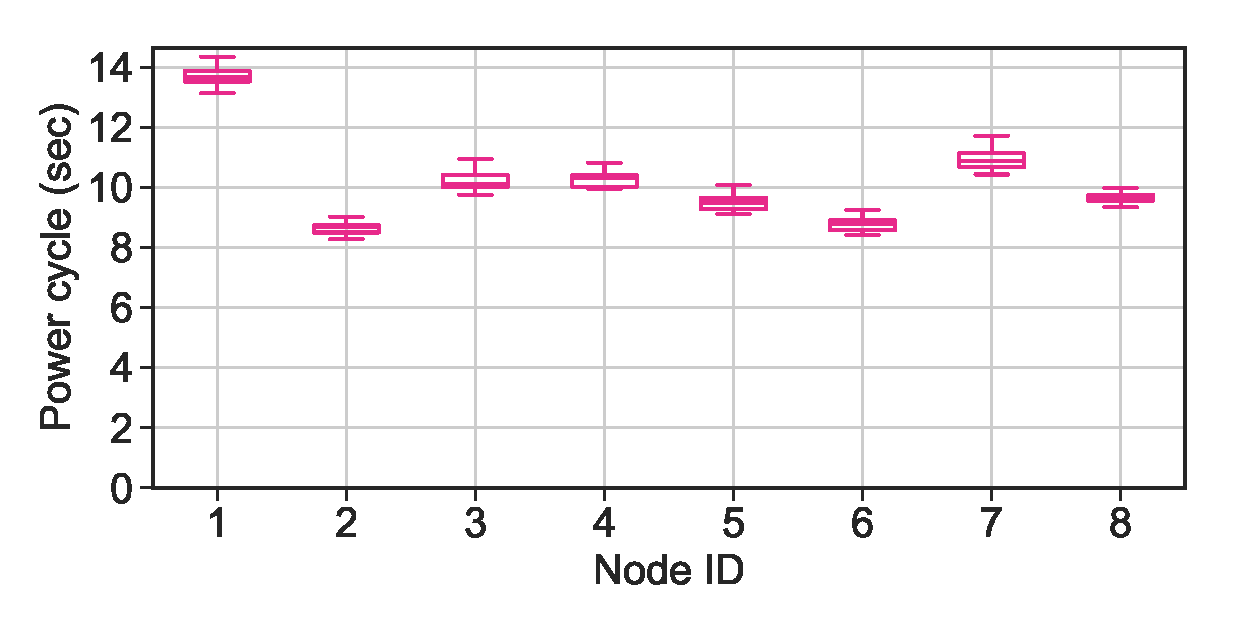
\includegraphics[width=\textwidth]{figures/light_power_cycles_len}
			\caption{Light}
		\end{subfigure}\hfill
		\begin{subfigure}{.49\columnwidth}
			\centering
			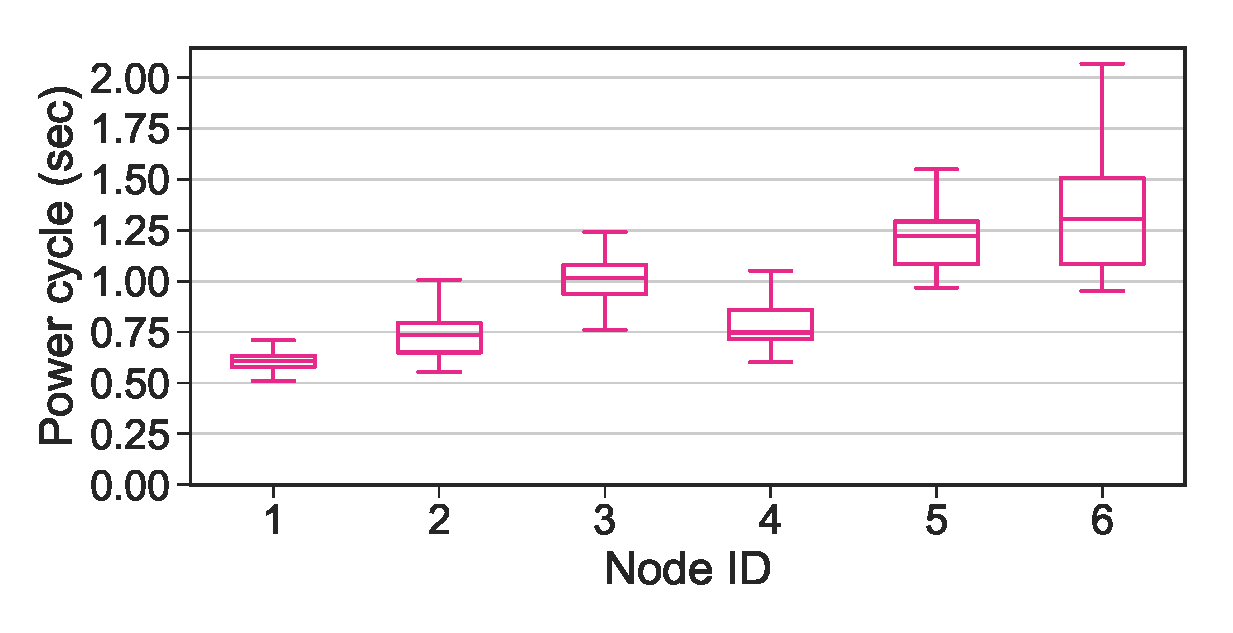
\includegraphics[width=\textwidth]{figures/rf_power_cycles_len}
			\caption{RF}
		\end{subfigure}\hfill
		\caption{Nodes' power cycles length for different energy sources, and different energy buffer sizes.}
		\label{fig:power_cycles}
\end{figure} 
%
\subsubsection{Events classification}
\label{sec:event_classification}
The availability of a \sys is not a single stretched interval: it is a chain of short intervals. Therefore, it is important to classify, from a \sys perspective, which types of events the \sys is best suited for. 
%
\begin{itemize}
\item \textit{Short events}: are events that can be captured using single intermittent node. For example, a spoken word can be seen as a short event if the energy needed to recorded is less than what the energy buffer, i.e., the capacitor, can store.
\item \textit{Long events}: are events that need more energy to be completely captured than what the energy buffer can store. They can be subdivided into three categories: 
	\begin{itemize}
		\item \textit{Simple}: is a long event that can be captured using single intermittent node---capturing part of it is sufficient to obtain all the information of interest---such as the sound produced by the friction between two moving parts of an engine. 
		\item \textit{Burst}: is a group of short events that requires multiple intermittent nodes to be captured such as a command of a few words (e.g., room temperature up).
		\item \textit{Complex}: is a long event that must be fully captured to be recognized. For example, sampling a gyroscope attached to a moving device (e.g., a toothbrush).

	\end{itemize}
\end{itemize}

Based on the above classification, we can argue that designing a \sys for long events is not like designing it for capturing short ones. While capturing a short event may require continuous \sys availability, capturing a long simple event that is longer than the power cycle $t_\text{p}$ does not require extending the availability of a single intermittent node. Furthermore, capturing a long complex event may require data fusion and processing that require the \sys{}s' nodes to communicate the raw data to a more powerful node, which may lead to significant overhead. However, this paper focuses on short and long bust events as they cover a wide range of applications (e.g., voice-controlled human-object interface). 
%ToDo what about the long smpile event (it is a relax version of the problem of capturing short event, i.e., less less stricked availability is required)

\subsubsection{Effective Availability}
%
\begin{figure}
		\centering
		\includegraphics[width=\columnwidth]{figures/effective_availability}
		\caption{Simulating the availability, the effective availability, and successfully captured events of a \sys of 10 nodes with a node duty cycle $\in \{10\%, 20\%,...,50\%\}$.}
		\label{fig:cis_simulation}
\end{figure}
%
Approaching continuous availability does not mean that a \sys can successfully capture all events. It can happen that an event is being only partially captured by one or more nodes, which may lead to unsuccessful event detection. Therefore, it is important to specify the effective availability of a \sys that leads to a successful event capturing (which we assume leads to successful sensing). 

\paragraph{polling-based Sensing}
Let us assume that we have a \sys of a single intermittent node monitors a short event of length $t_\text{e}$. For capturing the entire event, the event has to arrive within the interval, $t_\text{on} - t_\text{e}$, which we call, the effective on-time of an intermittent node.
Therefore, the effective availability of a \sys of $N$ nodes is the joined effective on-times of the underlying intermittent nodes, which can be modeled as,
%
\begin{equation}
		A_\text{v}(N) = A_\text{v}(N-1) + \left(1-A_\text{v}(N-1)\right) \times \frac{t_\text{on} - t_\text{e}}{t_\text{p}},
		\label{eq:cisSenseModel}
\end{equation} 
%

\paragraph{Event-driven Sensing}
An intermittent sensor has a limited energy budget per power cycle. When it is tasked with a polling-based sensing activity, its energy consumption, generally, switches between two levels: zero when charging and maximum when it activates its microcontroller for data acquisition and processing (Note that we assume that the microcontroller is the dominant energy consumer module of a node). However, in event-based sensing, a node puts its microcontroller into low-power mode and waits (or listens) for an external event to wake up the microcontroller. For example, in our prototype, a voice-controlled command recognizer, we exploit the microphone's wake-on-sound feature to send an interrupt to the microcontroller, which will then start recording the sound samples from the microphone. 
This wake-on-event style of operation is important as the minimal energy consumption during sleep significantly prolongs the period during which an event can be handled (for example, our prototype consumes 7 times less energy during sleep compared to being active).
To model the effective \sys availability when it is tasked with event-based sensing the change in energy consumption between the sleep and active mode must be taken into account. Since the event itself times when the node changes its energy consumption, we can model the effective availability as,
\begin{equation}
		A_\text{v}(N) = A_\text{v}(N-1) + \left(1-A_\text{v}(N-1)\right) \times \frac{t_\text{s} - (t_\text{e} \times\frac{e_\text{a}}{e_\text{s}}) }{t_\text{p}},\footnote{Notice that, there is a subtle point about equation~\ref{eq:cisEventSenseModel} as when an event arrives the node wakes up, consuming more energy. Therefore, its uptime shirnks. We, for similicity, modeled this effect by extending the events time with same factor. This is sufficient to say if the event will be fully captured or not (effective availability). However, if too many events arrives then the nodes will spend significant time in the active mode which changes the total availability of the system.}
		\label{eq:cisEventSenseModel}
\end{equation}

where $t_\text{s}$ is the expected sleep time of the \sys's nodes and $e_\text{a} and e_\text{s}$ are the energy consumption at active and sleeping modes, respectively.
%
\subsubsection{Simulation}
To do a first sanity check on our models, we simulated $10^5$ power cycles of a \sys of 10 nodes (Figure~\ref{fig:cis_simulation}). The duty cycles of the nodes range from $10\%$ to $50\%$, while the event length is fixed at $3\%$ of the power cycle length, $t_\text{p}$. The on-times and events arrivals were uniformly distributed over the power cycles. 
The results clearly confirm our models and support our argument about the distinction between \sys's availability and effective availability. The importance of this distinction is a function of the value $\frac{t_\text{e}}{t_\text{on}}$; observe the difference between availability and effective availability when nodes' duty cycle is $10\%$ (large effect) and $50\%$ (negligable effect).
%
%
\subsection{Environment}
Ambient energy controls the availability of a \sys's nodes.  Consequently, it also controls their collective response to external events. When it rises, it extends nodes' on-times. Extended on-times may cause node's power cycles to be synchronized on events arrival, compromising the \sys's overall availability. To overcome this problem the \sys's nodes must be power-state aware and able to estimate the number of active nodes in the \sys.
%
\subsubsection{Power States}
\label{sec:power_state}
A \sys can experience a wide range of ambient power intensities. For example, a solar-powered \sys may harvest no energy at night, modest energy from artificial light, and abundant energy from direct sunlight.  Generally, we can identify four different \sys powering states: 
\begin{itemize}
		\item \textit{Targeted power state}---These are the powering conditions that a \sys is designed for. In these  conditions, the \sys should work intermittently and have sufficiently randomized power cycles to uniformly distribute its intermittent nodes on-times and meet the desired availability (Figure~\ref{fig:cisModel}). In general, the targeted powering conditions should be near worst energy harvesting conditions to ensure that the system is properly functioning for the majority of the time.
		\item \textit{Under-targeted power state}---Ultimately, the ambient energy is an uncontrollable power source, and it is not hard to imagine scenarios where a \sys will be under-powered or even comes to complete and long power down (for example, a solar \sys will come to a perpetual power down in the darkness). In general, for under-targeted energy conditions, the \sys behavior can be considered as undefined.
%
\begin{figure}
		\centering
		\includegraphics[width=\columnwidth]{figures/hibernating_power_state}
		\caption{\fullsys is in a hibernating power state when the energy harvesting rate approximates the energy consumption rate at the sleeping (or low-power) mode. In this state, the intermittent nodes lose the randomization in their power cycles. Thus, all the nodes capture the same event and power down shortly after missing the subsequent ones. Consequently, the \sys senses intermittently and does not take advantage of its redundant intermittent nodes to approach continuous sensing.}
		\label{fig:noRand}
\end{figure} 
%
		\item \label{it:hibernating} \textit{Hibernating power state}---In event-based sensing scenarios, the intermittent nodes of a \sys sleep in low-power mode waiting for an external event to wake them up. If the energy conditions are relatively higher than the targeted conditions, the nodes may not die and sustain their sleeping power consumption. This will cause them to synchronize their wake-ups on the first incoming event and their power down as the event capturing process depletes their energy buffers quickly. Consequently, the \sys may miss the next incoming events (specially if the events happens to arrive in bursts) causing it to sense intermittently instead of continuously, see Figure~\ref{fig:noRand}. 
		%
		\item \label{it:continuous} \textit{Continuous power state}---Under direct mid-noon sun a tiny solar panel may provide sufficient power to run a sensor node continuously. In such conditions, the \sys will sense continuously without the need for randomization. Therefore, the job of a single node will be repeated $N$ times, and instead of sending a single message to a battery-powered or tethered sink---to push the data to the Internet---$N$ identical messages will be sent.
		These messages will collide as they are sent at about the same time, causing the information to be lost; if they arrive, however, they -except the first one- will waste energy of the sink as they carry the same information.  
		 % at about the same time causing them to collide or waste energy as they replicated the same information that has been delivered by the first message. 
				
\end{itemize}
%
The inefficiencies highlighted in the hibernating and continuous power states can be mitigated by enforcing randomization on the response of intermittent nodes 
% (Figure~\ref{fig:rand})
: when a node is woken up by an external event it responds to that event with a certain probability. However, if the randomized response is enforced all the time, then the \sys will have a lower probability of catching events during the targeted energy conditions state. Therefore, the \sys has to distinguish between the targeted and above-targeted energy conditions and randomize its response only during the hibernating and continuous power states. 

Choosing a fixed response probability is an inefficient way of dealing with the over-powering problem as the number of active intermittent nodes at a given moment is a function of the total number of intermittent nodes and the power intensity at that time. Therefore, efficient randomization requires intermittent nodes to estimate the number of active nodes and respond proportionally. Our proposed algorithm for estimating the number of active nodes depends on the nodes ability of measuring their on-times and off-times.

\subsubsection{Intermittent Timing}
\label{subsec:interTimer}
%
\begin{figure}[t]
		\centering
		\includegraphics[width=\columnwidth]{figures/softwareClock}
		\caption{The difference in the time of discharging the energy buffer---a node's on-time---when an energy-harvesting device is allowed to charge while operating, and when it is not allowed.}
		\label{fig:softwareClock}
\end{figure} 
\begin{algorithm}[t]
	\captionof{algorithm}{off-time estimation}
    \label{algo:offTime}
    \small
    \begin{algorithmic}[1]
		\State $R_\text{cntr}\text{++}$   \Comment{a persistent reboot counter} \label{lin:i}
			% \State $i \leftarrow $ \Call{$f_\text{reboot}$}{$i$} \Comment{$i$ is a persistent variable} \label{lin:i}
		\State $E_\text{buf}$ \Comment{Size of energy buffer}
		\State $t_\text{a}$ \Comment{time of discharging $E_\text{buf}$ at load $a$, no harvesting}\label{lin:ta}
		\State$ X_\text{cy} $ \Comment{time every $X$ power cycles} 
		\LeftComment{\colorbox{lightgray}{Code executed on each $X$ power cycles \hspace{3cm} }}
		\If{$(R_\text{cntr} == X_\text{cy})$}
		    \State $R_\text{cntr}=-1$
			\State \Call{$f_\text{load}$}{$a$} \Comment{set node load to $a$ } \label{lin:fixedLoad}
			\State $t_\text{on} \leftarrow$ \Call{time}{\null} \Comment{measure time until power down}\label{lin:ton}
		\EndIf
		\LeftComment{\colorbox{lightgray}{Code executed on each $X+1$ power cycles \hspace{2.5cm}}}
		\If{$(R_\text{cntr} == 0)$}
			\State \label{lin:deltat}$\Delta{t} = t_\text{on}-t_\text{a}$  \Comment{time difference due to charging} \label{lin:td}
			\State \label{lin:ehar}$E_\text{har} \leftarrow E_\text{buf}\times \frac{t_\text{a}}{\Delta{t}}$ \Comment{harvested energy}
			\State $P_\text{in} \leftarrow E_\text{har}\div{t_\text{on}}$ \Comment{incoming power} \label{lin:pin}
			\State \label{lin:offtime}$t_\text{off} \leftarrow E_\text{buf}\div P_\text{in}$ 
		\EndIf
	\end{algorithmic}
\end{algorithm}
%
Timing is a key building block of sensing systems. It is, however, missing on intermittent nodes unless an additional dedicated (RC-based) timer is added to them~\cite{hester2017timely}. Here we would like to propose an alternative that does not require additional hardware. This alternative does not only enable time estimation but also ambient energy richness, which is very important for estimating the number of a node's active neighbors. But, \textit{how a node can time its own on/off cycle?}

Intermittent nodes fail abruptly; therefore, a persistent timer is needed. A simple way to emulate persistent timer is by using a persistent counter, or sampling the volatile built-in timers of the microcontroller and save the obtained values in the non-volatile memory. To estimate the off-time, $t_\text{off}$ in Figure~\ref{fig:softwareClock}, a node needs to determine the incoming power (harvesting rate). The average harvesting rate can be induced from the on-time as follows.
%
The node measures its on-time while harvesting, see $t_\text{on}$ in Figure~\ref{fig:softwareClock}, and compares it to the time required to drain the energy buffer \emph{without} charging, see $t_\text{a}$ in Figure~\ref{fig:softwareClock}. The additional on-time, $\Delta t$, is the result of the energy accumulated while executing. 
%
If $t_\text{on}$ and $t_\text{a}$ are measured on the same load---thus, they have the same power consumption---then the amount of the energy harvested while the device is on can be calculated as in Line~\ref{lin:ehar}, Algorithm~\ref{algo:offTime}. And, the average input power can be found as in Line~\ref{lin:pin} that, in turn, enables the node to estimate its own $t_\text{off}$ (Line~\ref{lin:offtime}).
Since calculating the off-time requires constant load, the sensor cannot run arbitrary code during time measurement. Therefore, the sensor needs to sacrifice a certain percentage of its power cycles for time measurement, Line~\ref{lin:i}-\ref{lin:ton}. Once the on-time and off-time are found the node's power cycle for load $a$ is determined.

\subsubsection{Nodes overlapping}
\begin{figure}[t]
		\centering
		\begin{subfigure}{.49\columnwidth}
			\centering
			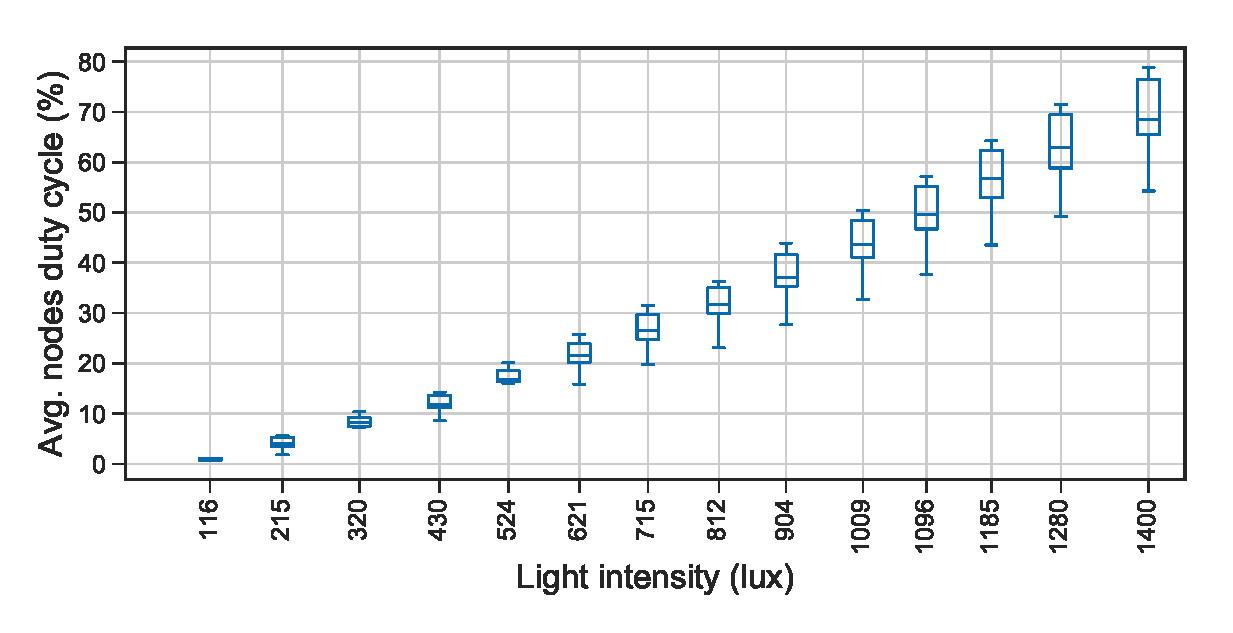
\includegraphics[width=\textwidth]{figures/cis_dutyCycle}
			\caption{Light}
		\end{subfigure}\hfill
		\begin{subfigure}{.49\columnwidth}
			\centering
			\includegraphics[width=\textwidth]{figures/rf_cis_dutyCycle}
			\caption{RF}
		\end{subfigure}\hfill
		\caption{The average duty cycles of 8 solar-powered and 6 RF-powered intermittent nodes for different ambient energy sources and energy intensities. In general, the average duty cycle of a node is a good indicator of the average duty cycle of \sys's nodes.}
		\label{fig:cis_nodes_dutyCycle}
\end{figure} 

\begin{table}
		\centering
		\caption{Measuring intermittent nodes overlapping of a \sys of 8 intermittent nodes for different light intensities.}
		\begin{tabular}{lll}
				\hline
				\textbf{light (lux)} & \textbf{$N_\text{active}$} & \textbf{std}   \\
				\hline
				300	                  & 1.01 & 0.85   \\
				500                   & 1.63 & 0.98   \\
				800                   & 2.88 & 1.50   \\
				1200                  & 5.05 & 1.08   \\
				\hline
		\end{tabular}
		\label{tab:clusters}
\end{table}
% In order for a node to estimate the number of active nodes at a given moment, first, it has to know the total number of nodes ($N$) in its \sys, which we assume to be known to the nodes before deployment. Second, this analysis is built on the observation that a node's on-time is a good indicator about the on-times of other nodes in the \sys, see Figure~\ref{fig:cis_nodes_dutyCycle}. A node can measure its on-time $t_\text{on}$ and off-time $t_\text{off}$ using  Algorithm~\ref{algo:offTime} (or an external dedicated timer~\cite{hester2017timely}). 

Now, a \sys's node has all the information needed to estimate the number of active nodes in its \sys. Namely, it knows

In order for a \sys's node to estimate the number of active nodes at a given moment, it needs to determine the following information: 
\begin{enumerate*}[label=(\roman*)]
 \item the size of the \sys it belongs to, which is a constant value that can be loaded to the memory; 
 \item its own $t_\text{on}$ and $t_\text{off}$; and 
 \item how the \sys's nodes' on-times are distributed, Model~\ref{eq:cisModel}.
\end{enumerate*}
% Notice that, on/off times of a \sys's node can be used to estimate other \sys's nodes' on/off times.
% This is intuitively valid as the nodes have the same energy buffer size and are expose to the approximately the same energy conditions~\footnote{}. 
Figure~\ref{fig:cis_nodes_dutyCycle} shows the average power cycles of solar- and RF-powered nodes.
We can conclude from these measurements that a node power cycle approximates other \sys's nodes power cycles.
This observation can be generalized by considering that the nodes of a \sys are assumed to have the same energy buffer size and they are in a close proximate, and therefore, they are expose to roughly the same energy conditions (this should not be confused with argument about the emerging uniform distribution of nodes' on-times as this distribution appears due to \emph{small} differences between the power cycles).  

Now, a node can estimate the maximum time span ($t_\text{max}$) of its \sys, which is the total duration of the nodes' on-times when they are aligned next to each other, as follows
\begin{equation}
t_\text{max} = N\times t_\text{on}.
		\label{eq:max_time}
\end{equation}
Then, from Equation~\ref{eq:cisModel}, the node calculates the \sys availability ($A_\text{v}(N)$). As we argued in Section~\ref{subSec:availability}, nodes on-times are uniformly distributed over the longest power cycle, $t_\text{p}^\text{max}$. Thus, the overlapping on-time is also uniformly distributed. Then, the node can calculate the average number of active intermittent nodes $N_\text{active}$ using the following formula,
\begin{equation}
	N_\text{active} = \frac{t_\text{max}}{t_\text{p}^\text{max}\times A_\text{v}(N)}.
	\label{eq:active}
\end{equation}
and choose the proper randomization factor. If a second event, however, happens shortly after the first one, a node needs to update $N$ as follows, 
$$
N = N - (N_\text{active}-1)
$$
the $-1$ is because the node itself decided not to react on the first event. 

Table~\ref{tab:clusters} shows the average number of overlaps of an 8-nodes \sys for different light intensities. These measurements validate that nodes overlapping time is uniformly distributed over the \sys on-time. For example, at $\SI{1200}{lux}$ an individual node of our \sys has a duty cycle of $\approx$\,62\%. If we multiply it by the number of nodes (Equation~\ref{eq:max_time}) we get about 500\%. Figure~\ref{fig:cisModel} indicates that a \sys with eight nodes of duty cycles above 50\% has near 100\% availability. From equation~\ref{eq:active}, we find that the expected number of clustered nodes is 5 which is what Table~\ref{tab:clusters} also shows. 









































%\section{Distributed Intermittent System} 
\section{Prototype: Coalesced Intermittent Command Recognizer}
\label{sec:disMic}
\begin{figure}
	\centering
	\includegraphics[width=\columnwidth]{figures/cis}
	\caption{\fullCIM: an instant of a \fullsys. \cim features a power failure immune word recognizer. Once a word is recorded, the word's spectral features extraction begins. The resulting features vector is compared against previously-stored words' templates for recognition. The comparison using a liner distance matching algorithm}
	\label{fig:cis}
\end{figure}

We have developed a prototype of a \fullcim (\cim): an instant of a \fullsys. The \cim consists of eight batteryless intermittent nodes. Each node is capable of performing isolated words recognition. 

The reason behind developing a \cim is threefold: (i) voice is a natural and convenient way for human to interact with miniaturized devices; (ii) demonstrating \textit{the world's first} batteryless intermittently-powered command recognizer, which shades light on the potential of batteryless intermittent systems; and (iii) facilitating testing with different sensing strategies and different type of external events arrival (i.e., regular  or burst). 


% Moreover, we believe that a \cim can facilitate direct human-to-human or human-to-objects communication. Imagine that a \cim based system is deployed in a play ground, embedded in ground and other objects. You want to call your child, and a \cim based system is embedded in your shirt and his shirt. You say his name and the \cim picks up the word and scatter it over light---\cite{marco}  demonstrates the feasibility of scattering sunlight to communicate between two nodes that are up to 60\,m apart. The scattered signal will be relied on other \cim nodes until the receiving node on his shirt receives the message and notify him, daddy is calling. 

\subsection{Hardware}
\label{sec:hardware}
A \cim node consists of thee main parts: a microphone, a microcontroller, and a harvester. MSP430RF5994~\cite{ti_msp430_website}, an ultra-low-power microcontroller, is used for data acquisition and processing. This microcontroller has a 16-bit RISC processor running on 1 MHz, 8KB of SRAM (volatile), 256KB of FRAM (non-volatile), and a 12-bit analog to digital converter (ADC). It also features a Low Energy Accelerator (LEA), which offloads the main CPU for specific operations, such as FFT. For recording we use the PMM-3738-VM1010-R piezoelectric MEMS microphone, which features Wake on Sound and ZeroPower listening technologies \cite{microphone}, allowing both the microcontroller and the microphone to sleep in a low-power mode until a sound wave is detected.
The microcontroller and microphone are powered by a BQ25570 solar power harvester~\cite{BQ25570EVM-206_website} connected to an IXYS SLMD121H04L solar cell~\cite{SLMD121H04L_website} and a super-capacitor of 470 \si{\micro F}. For debugging we used the Saleae logic analyzer~\cite{saleae}.

\subsection{System Description}
The \cim has a power interrupts immune command recognizer. The recognizer is capable of recognizing isolated-word type of speech. 
The main parts of the recognizer are illustrated in Figure~\ref{fig:cis} and explained below:

\subsubsection{Data acquisition}
The \textit{Wake-on-Sound} feature of the microphone triggers the data acquisition process once the energy level in the sound signal crosses a certain level. The ADC, then, samples the output of the microphone at 8\,kHz. This sampling rate is sufficient to cover most of the frequency range of the human voice. To determine the end of the recording we relied on the characteristics of the targeted vocabulary. In particular, we identified experimentally the minimum effective recording length, which is 
%happened be 
285\,ms for the chosen set of words. By exploiting the Wake-on-Sound feature and using the minimum effective recording length, we eliminate the need for an endpoint detection algorithm, greatly improving the processing time and system efficiency from the energy perspective.


\subsubsection{Feature Extraction}
Once a recording has finished, framing and data processing begin. \cim divides the digitized signal into non-overlapping frames of 256 samples ($\approx$ 33 milliseconds). This size is beneficial for doing a Fast Fourier Transform and short enough for the voice-features to be considered constant inside a frame.

To extract the spectral features of a frame, \cim divides the frequency of interest into 12 bands (as in~\cite{hopper1992}). The first five bands has a bandwidth of 200\,Hz. The next three has a bandwidth of 300\,Hz which is followed by two bands of 500\,Hz. Finally, the last two bands has a 600\,Hz bandwidth. This division is motivated by how the energy is concentrated in human speech~\cite{hopper1992}. Then, \cim computes the 256-point Fast Fourier Transform for each frame. The resulting feature vector contains the amount of energy concentrated in each frequency band defined earlier. This feature vector forms the basis for the words identifying process once it is normalized.

We normalize the feature vectors to minimize detection errors that result from differences in the amplitude of the speech input. To normalize a feature vector, \cim computes the binary logarithm of each entry of that vector. 
Then it computes the mean of the resulting vector. Finally, it subtracts the computed mean from each entry of the resulting vector. This is summarized in the following equation: 
\begin{equation}
    f_i = \log(\hat{f}_i) - \frac{\sum\limits^S_{i=1}\log(\hat{f}_i)}{S},
\end{equation}
where $f_i$ is the normalized output for the $i^{\text{\tiny th}}$ spectral band of a feature vector, $\hat{f}_i$ is the energy in the $i^{\text{\tiny th}}$ spectral band of the frame, and $S$ is the number of spectral bands (12 in our case). 

\subsubsection{Feature Matching}
% %
% \begin{figure}
% \centering
% 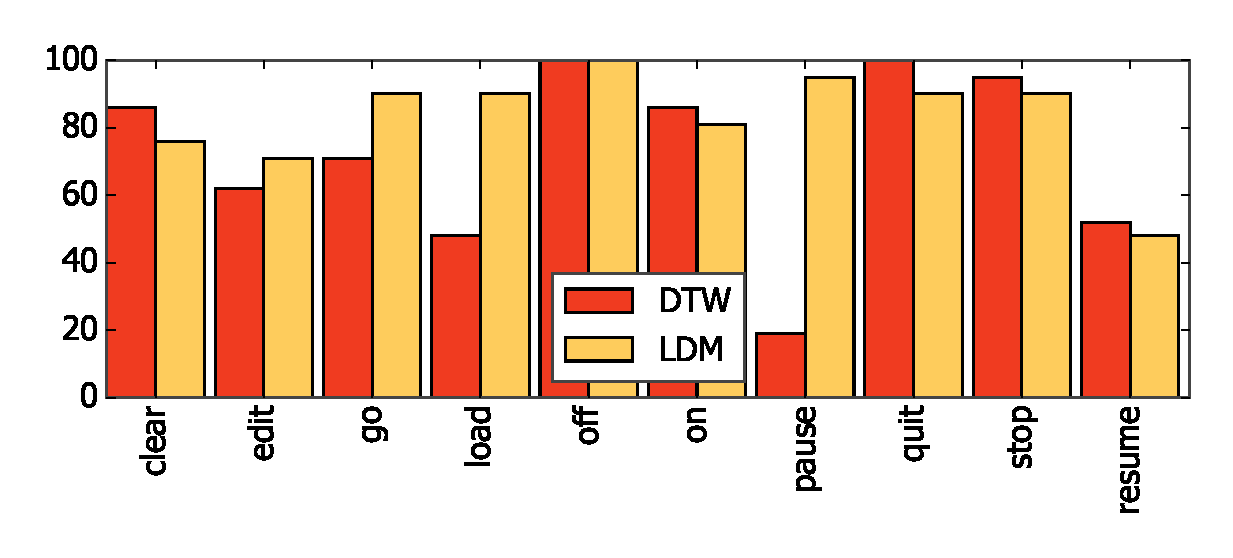
\includegraphics[width=\linewidth]{figures/DTWvsLDM}
% \caption{Recognition accuracy for linear matching and DTW when using 9 frames as the recording length.}
% \label{fig:DTWvsLDM}
% \end{figure}
% %
\begin{table}
	\centering
	\caption{Profiling of features matching algorithms: Dynamic Time Warping (DTW) and Linear Distance Matching (LDM)}
	\label{tab:profiling}
	\begin{tabular}{lll} \hline
	Section & LDM (ms) & DTW (ms) \\\hline
	Recording & 285  & 285 \\
	Feature extraction & 501 & 501 \\
	Feature matching &  99 & 1251 \\\hline
	Total & 885 & 2037 \\\hline
	\end{tabular}
\end{table}
%
Feature matching is achieved by computing the distances between the normalized feature vectors of the recorded word and the feature vectors of the words stored during the training phase (templates). 
\cim computes the squared Euclidean distance between vectors as follows:
\begin{equation}
	 	d_j = \sum\limits^S_{i=1} (f_{s,i} - f_{r,i})^2,
    \label{eq:frame_dist}
\end{equation}
where $d_j$ is the distance between the $j^{\text{\tiny th}}$ stored and recorded vectors. $f_{s,i}$ is the normalized output of the $i^{\text{\tiny th}}$ spectral band of a stored vector, $f_{r,i}$ is the normalized output of the $i^{\text{\tiny th}}$ spectral band of a recorded vector. 
The total distance between two words is calculated as follows:
\begin{equation}
		D_k = \sum\limits^{l}_{j=1} d(j)
\end{equation}
where $D_k$ is the distance between the $k^{\text{\tiny th}}$ stored word and the recorded word, and $l$ is the recording length measured in frames.

Once the recorded word has been compared to all \cim template words, the template with the smallest distance to the recorded word is considered the correct word. However, if the smallest distance is bigger the garbage threshold which we experimentally set, then the \cim will return "undefined word". 

It should be emphasized that in linear distance matching (LDM) the feature vectors of two words are compared successively, not accounting for differences in pronunciation speed. This is sufficient for our case as we are targeting isolated words and speaker dependent speech recognition type. We also implemented the Dynamic Time Warping algorithm which better handles the difference in the speed of speech. However, it is slower than the linear matching algorithm  (Table~\ref{tab:profiling}) and the detection accuracy was comparable in our case.% (Figure~\ref{fig:DTWvsLDM}). 

\subsubsection{Power Failure Protection}
In order to preserve the progress state and to protect \cim data against randomly timed power failures, we manually split \cim program into 19 atomic regions. We ensured the each of these regions requires less energy then what the energy buffer can provide with a single charge. The program progress state is saved in the non-volatile memory (FRAM) on the transition between these regions. This prevents the program from falling back to its starting point (\texttt{main()}) after each power failure. Data in the non-volatile memory with Write-After-Read dependency is double buffered to ensure data integrity when the power supply is interrupted. 

\subsection{Code profiling}
The entire command recognition software was written in the {\tt C} programming language. The total program consists of 973 lines of code, excluding the FFT function from the Texas Instrument DSP library. See Table~\ref{tab:code_stats} for more information.

The memory footprint on the microcontroller is 20,064 bytes of FRAM and 1,134 bytes of SRAM. Execution times are shown in Table~\ref{tab:profiling}.

The power usage of a node differs according to it's activity. When a node is waiting for a voice event, it is in low-power mode. When data needs to be processed or recorded it is in active mode. When recording, the microphone and ADC consume additional power. The power consumption rates are determined by measuring the current with a Monsoon power monitor~\cite{monsoon} and shown in Table~\ref{tab:power_usage}.


\begin{table}
	\centering
	\caption{Code statistics: lines of code}
	\label{tab:code_stats}
	%Compiled without optimization flags:
	\begin{tabular}{lrrrr} \hline
		Language & Files & Blank & Comment & Code \\\hline
		C & 7 & 264 & 173 & 736 \\
		C/C++ Header & 8 & 62 & 40 & 237 \\\hline
		Total &  15 & 326 & 213 & 973 \\\hline
	\end{tabular}
\end{table}

\begin{table}
	\centering
	\caption{Power usage.}
	\label{tab:power_usage}
	%Compiled without optimization flags:
	\begin{tabular}{lrrr}\hline
	Section & Current (\si{\micro A}) & Voltage (V) &  Power (\si{\micro W}) \\\hline
	Sleeping & 64 $\pm$20 & 2.008 & 128 $\pm$40 \\
	Recording & 423 $\pm$20  & 2.008 &  849 $\pm$40\\
	Processing &  282 $\pm$20 & 2.008& 566 $\pm$40 \\\hline
	\end{tabular}
\end{table}

\section{Evaluation}
\label{sec:evaluation}
\begin{table}[H]
\centering
\caption{Testing set}
\label{tab:words}
\begin{tabular}{lllll}
\hline
on    & off  & stop & clear & load   \\
go & pause & resume & edit  & quit  \\  
\hline  
\end{tabular}
\end{table}

\subsection{Effective recording length}
\label{subsec:rec_length}
%
\begin{figure}
	\centering
	\includegraphics[width=\linewidth]{"figures/linear_multi"}
	\caption{Recognition accuracy versus the recording length (in frames), while using multiple recordings per word for testing. Used feature matching method: linear.}
	\label{fig:multi}
\end{figure}
%
Since our target hardware has extremely limited resources, the first experiment targets the minimum effective recoding length without significant accuracy loss. 

For this experiment a single microcontroller running on continuous power is used. Each word from Table~\ref{tab:words} was recorded on a PC 20 times. The features---normalized FFT-based values---of the first recording are saved in the microcontroller's persistent memory as a signature to perform the feature matching, during the testing. the rest of the recording are used for conducting the experiment.   

Figure~\ref{fig:multi} shows words recognition accuracy when the 19 recordings of each word are played back from the PC speaker. We can concluded that recording beyond \textit{nine frames} do not increase the recognition accuracy; therefore, nine frames recording length is chosen for the rest of the experiments. 

\subsection{Comparison of feature matching methods}
%
\begin{figure}
\centering
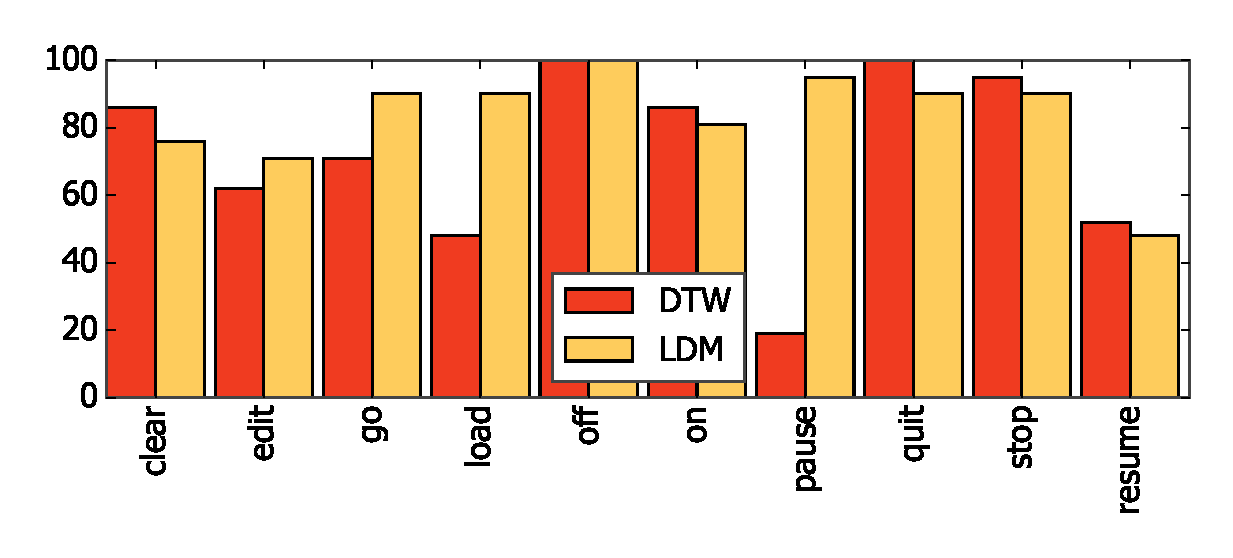
\includegraphics[width=\linewidth]{figures/DTWvsLDM}
\caption{Recognition accuracy for linear matching and DTW when using 9 frames as the recording length.}
\label{fig:DTWvsLDM}
\end{figure}
%
\begin{table}
	\centering
	\caption{Profiling of features matching algorithms: Dynamic Time Warping (DTW) and Linear Distance Matching (LDM)}
	\label{tab:profiling}
	$
	\begin{tabular}{lll}\hline
	Section & Linear (ms) & DTW (ms) \\\hline
	Recording & 285.9  & 285.9 \\
	Feature extraction & 501.9 & 501.9 \\
	Feature matching &  99.4 & 1251 \\\hline
	Total & 887.2 & \\\hline
	\end{tabular}
	$
\end{table}
%
We implemented two algorithms for voice features matching, Dynamic Time Warping (DTW) and Linear Distance Matching (LDM). Due to the microphone wake-on-sound feature and the fixed recording length, DTW did not outperform LDM as Figure~\ref{fig:DTWvsLDM} shows. Moreover, DTW takes more time to process that data as Table~\ref{tab:profiling} shows. Therefore, LDM algorithm is used in future experiments.

\subsection{ Intermittent microphone availability}
%

\begin{figure}
\centering
\includegraphics[width=\linewidth]{figures/word_freq}
\caption{The effect of the time between consecutive words on the availability: the percentage of words that is processed by the command recognizer. \todo{Add correct recognition as stacked bar?}}
\label{fig:word_freq}
\end{figure}
%
\begin{table}
	\centering
	\caption{The mean and standard deviation of the parameters that were used to simulate intermittent execution. Here $t_{on}$ is the time the device is on while recording or processing, $t_{off}$ is the time the device is charging and $t_{sleep}$ is the time the device is sleeping while waiting on sound input.}
	\label{tab:simparams}
$
\begin{array}{lll}\hline
\text{Parameter} & \mu \text{ (ms)} & \sigma \text{ (ms)} \\\hline
%t_{rec} & 295 & 0 \\
t_{on} &  590 & 17.7 \\
t_{off} & 5310 & 154 \\
t_{sleep} &  22420 & 652 \\\hline
\end{array}
$
\end{table}
%
This experiment shows the effect of intermittent power supply on a microphone availability \todo{and recognition accuracy} for different command (or word) repetition speed. Each word (from Table~\ref{tab:words}) was played back 20 times with intra-words-playing time ranges from 1 to 10 seconds. 

For the experiment we chose to simulate the intermittent power supply, based on a real measurement, to ensure environment consistency across different words.
In particular, we measured the $t_{on}$; used an on/off ratio of $10\%$ to simulate harsh harvesting conditions~\cite{mementos, harvOS,lucia}; and calculated the $t_{sleep}$ based on the micro controller specification~\cite{datasheet} (Table~\ref{tab:simparams}).     

The obvious observation from Figure~\ref{fig:word_freq} is that intermittency has a great impact on the command recognizer availability. However, a less obvious, but important, observation is that the correlation between the on/off cycle and the command repetition speed has also great impact as the bars labeled with 5 and 6 from Figure~\ref{fig:word_freq} indicate. 








% \section{Discussion }
% \label{sec:discussion}
% \begin{figure}

	\begin{subfigure}{0.49\columnwidth}
		\includegraphics[width=\textwidth]{figures/BatterylessNodesDutyCycles_Active_mode}
		\caption{The node powers up and goes into active mode. The high energy consumption rate at this mode makes the changes in the on-time due to changes in ambient energy very small. }
	\end{subfigure}\hfill
	%
	\begin{subfigure}{0.49\columnwidth}
		\includegraphics[width=\textwidth]{figures/BatterylessNodesDutyCycles_Sleep_mode}
		\caption{The node powers up and goes into sleep mode. The low energy consumption rate at this mode makes the changes in the on-time when ambient energy changes clearly noticeable. }
	\end{subfigure}
	\caption{On-times, off-times, and power (charge-discharge) cycle of a batteryless energy-harvesting node.)}
	\label{fig:pwrCycleVSEnergyIntensity}
\end{figure}

\paragraph{Different energy harvesting rates}
It can happen that some of the nodes of a \cis be in the shadow while the rest is under direct sunlight (e.g., when curtains are being opened). 
As a consequence, nodes' power cycles will generally be significantly different (Figure~\ref{fig:pwrCycleVSEnergyIntensity} shows the on-times, off-times, and power cycles when the ambient energy ranges from 400 to 1400\,lux). Therefore, nodes will not be able to accurately estimate the collective availability of the system, which reduces the overall performance. 
Taking into consideration that energy density vary overtime (e.g., the shadow of a curtain moves as the relative position of the curtain to the sun changes), an averaging technique might mitigate the negative effect of non-uniform distribution of ambient energy. 

\paragraph{Using machine learning algorithms to improve intermittent sensing}
In the future we plan to dive deeper in studying partially captured data. 
Intermittent sensors may partially capture events. Classical recognition 
algorithms face difficulties dealing with partially captured data. 
Therefore, we want to investigate \emph{how much machine learning algorithms 
can improve the sensing quality of intermittent sensing?} 
% \todo{MAC for backscattering and favorable energy conditions}




\section{Conclusion and Future Work}
This paper addresses the availability problem of intermittent sensors
that fail to capture (and process) events while charging their energy
buffer.  As the power to drive a node is much higher than what can be
harvested from ambient sources, the chance of capturing an event can
be as low as just 8\% (sunlight) and 4\% (RF) (cf.\ the duty cycles
reported in Figure~\ref{fig:cis_nodes_dutyCycle}). To address this problem of missing
most events we presented the \fullcis (\cis),
which is the abstraction of a group of intermittently-powered sensors,
whose collective duty cycle (on-time) can approach the desired 100\%
availability.  The inherent differences in the powering subsystem of
intermittent sensors result in (slight) differences in the sensor nodes'
power cycles causing the nodes' on-times to be uniformly distributed. This
implies that simply selecting the right number of nodes is all that
is required. To this end we have modeled the (effective) availability
of a \cis and validated its accuracy against data collected on real
hardware.

Experimentation with an 8-node prototype \cis, a basic voice-control
application recognizing up to 4-word commands, showed that the inherent
randomization in the power cycles can easily be disrupted. In case the
ambient power exceeds the (worst-case) design point and nodes employ an
efficient wake-on-event sleep mode, all nodes wake-up on the same (rare)
event. If the energy buffer is small then they all enter the charging
state at approximately the same time (unwanted synchronization) and
subsequent events (words) will be missed (compromising availability).
To counter this unwanted behavior, we proposed to use a probabilistic
approach in which the number of active neighbors is determined and nodes
respond proportionally to an event. This approach was shown to be effective
for our prototype, capturing burst events with above 85\% detection accuracy.

% Using machine learning algorithms to improve intermittent sensing
In the future we plan to dive deeper in studying partially captured data. 
Intermittent sensors may partially capture events. Classical recognition 
algorithms face difficulties dealing with partially captured data. 
Therefore, we want to investigate \emph{how much machine learning algorithms 
can improve the sensing quality of intermittent sensing?} 


% Energy-harvesting battery-less sensors can operate very long because their power source is unlimited. 
% However, ambient power is weak and volatile; therefore, these sensors operate intermittently.
% The intermittent availability compromises their value as they have a high probability of missing events. 
% This paper addresses the \emph{availability} problem of intermittent sensors. 
% %
% It presents the \textit{\fullcis} (\cis), which is the abstraction of a group of intermittently-powered sensors.
% A \cis is able to approach continuous sensing by taking advantage of the embedded randomization in the powering subsystem of intermittent sensors.
% The resulting differences in the sensor nodes' power cycles make the nodes' on-times uniformly distrusted. 
% Therefore, the number of a \cis nodes can be seen as a design parameter to achieve a targeted collective availability. 
% % Therefore, adding more nodes to a \cis increases its expected availability. 
% We have modeled the availability of a \cis and its effective availability: the availability that leads to successful event capturing. 
% Further, we showed the accuracy of these models by validating them against data collected on real hardware and with different ambient energy sources (i.e., sunlight, artificial light, and RF). 
% %
% Furthermore, we showed how the variation in nodes' power consumption and harvesting rate and the arrival of external events can compromise the \cis's availability (nodes employing sleeping mode to increase the chance of successfully capturing an event, synchronize their power cycles on the first incoming event, in a burst, and miss the subsequent ones. The probability of this unwanted synchronization increases when ambient energy rises beyond the design point.  
% % It taking advantage of the embedded randomization in the powering subsystem of energy-harvesting battery-less sensors to distribute
% % the on-times of a group of intermittent sensors uniformly in time 
% % We presented the \textit{\fullcis} (\cis), an intermittently powered ``sensor'' that senses continuously! \cis is built around the observation that multiple intermittent nodes distribute themselves uniformly in time. This observation enables us to accurately model, and validate on real hardware, the \cis availability---the collective on-time of its intermittent nodes. 
% % An important finding is that favorable energy conditions may cause sleeping intermittent nodes to synchronize their power cycles on the arrival of the first event. Consequently, they react to the same event, start recharging at the same time, and missing the next event. 
% % 
% To counter this unwanted behavior, we designed an algorithm to estimate the number of active neighbors and respond proportionally to an event. 
% We developed a prototype of the \cis, an 8-nodes \fullCIM (\cim). 
% Using this prototype, we showed that the \fullcis is able to distribute bursts of events on its nodes "evenly" and capture the entire burst with above 85\% detection accuracy.
 

% Intermittent sensors will partially capture events. Classical algorithms for recognizing and classifying these events might face difficulties  dealing with partially captured data. Thus, follow-up work can investigate \emph{how much machine learning algorithms can improve the sensing quality of intermittent sensing?} 
% Additionally, the command recognition rate could further be improved by using an estimation of the energy left in the energy buffer, to start recharging early. This will prevent a detection when there is not enough harvested energy to record for a long enough time, letting a node recharge earlier and coming back with sufficient energy.


% \noindent\textbf{Speech Recognition on Intermittent Devices} In this paper, we have shown the feasibility of speech recognition on intermittent power. We also demonstrated the possibility of recognizing burst of events (in our case four words). However, the type of speech we targeted is the simplest, isolated words. Next, we may attempt recognizing a more complicated type of speech and for a larger number of words than the number chosen for this study.




\section{Acknowledgements}
We like to thank Stephan Wong for his contributions in the early stages of this
work, and the anonymous referees for their comments helping us to polish the
paper to perfection.



\bibliographystyle{IEEEtran}
\bibliography{references}

\end{document}
